% This is "sig-alternate.tex" V1.9 April 2009
% This file should be compiled with V2.4 of "sig-alternate.cls" April 2009
%
% This example file demonstrates the use of the 'sig-alternate.cls'
% V2.4 LaTeX2e document class file. It is for those submitting
% articles to ACM Conference Proceedings WHO DO NOT WISH TO
% STRICTLY ADHERE TO THE SIGS (PUBS-BOARD-ENDORSED) STYLE.
% The 'sig-alternate.cls' file will produce a similar-looking,
% albeit, 'tighter' paper resulting in, invariably, fewer pages.
%
% ----------------------------------------------------------------------------------------------------------------
% This .tex file (and associated .cls V2.4) produces:
%       1) The Permission Statement
%       2) The Conference (location) Info information
%       3) The Copyright Line with ACM data
%       4) NO page numbers
%
% as against the acm_proc_article-sp.cls file which
% DOES NOT produce 1) thru' 3) above.
%
% Using 'sig-alternate.cls' you have control, however, from within
% the source .tex file, over both the CopyrightYear
% (defaulted to 200X) and the ACM Copyright Data
% (defaulted to X-XXXXX-XX-X/XX/XX).
% e.g.
% \CopyrightYear{2007} will cause 2007 to appear in the copyright line.
% \crdata{0-12345-67-8/90/12} will cause 0-12345-67-8/90/12 to appear in the copyright line.
%
% ---------------------------------------------------------------------------------------------------------------
% This .tex source is an example which *does* use
% the .bib file (from which the .bbl file % is produced).
% REMEMBER HOWEVER: After having produced the .bbl file,
% and prior to final submission, you *NEED* to 'insert'
% your .bbl file into your source .tex file so as to provide
% ONE 'self-contained' source file.
%
% ================= IF YOU HAVE QUESTIONS=======================
% Questions regarding the SIGS styles, SIGS policies and
% procedures, Conferences etc. should be sent to
% Adrienne Griscti (griscti@acm.org)
%
% Technical questions _only_ to
% Gerald Murray (murray@hq.acm.org)
%===============================================================
%
% For tracking purposes - this is V1.9 - April 2009

\documentclass{sig-alternate-2013}

\usepackage{subfigure}
\usepackage{graphicx}

\usepackage{url}
\usepackage{amsmath}
%\usepackage{breakurl}
\usepackage{multicol}
\usepackage{fancyvrb}
\usepackage{float}
\usepackage{xcolor}
\usepackage{array}
\usepackage{multirow}
\usepackage{tabularx}
\usepackage{colortbl}
\usepackage{hhline}
%\usepackage{authblk}

\usepackage[T1]{fontenc}
\usepackage[utf8]{inputenc}
\usepackage{lmodern}

\hyphenation{Web-Cite}
\hyphenation{Java-Script}
\hyphenation{local-host}
\hyphenation{Arch-ive-it}
\hyphenation{Arch-ive-It}
\hyphenation{Ar-chive}
\hyphenation{Time-Map}
\hyphenation{Time-Maps}
\hyphenation{Mem-ento}
\hyphenation{Date-time}
\hyphenation{Date-times}
\hyphenation{date-time}
\hyphenation{date-times}
\hyphenation{style-sheet}
\hyphenation{Style-sheet}
\hyphenation{style-sheets}
\hyphenation{Style-sheets}
\hyphenation{Mem-ento-Date-times}
\hyphenation{Mem-ento-Date-time}
\hyphenation{local-host}
\hyphenation{Ar-chive}
\hyphenation{app-li-ca-tion-like}
\hyphenation{Java-Script-de-pend-ent}

%\makeatletter
%\let\@copyrightspace\relax
%\makeatother

\newfont{\mycrnotice}{ptmr8t at 7pt}
\newfont{\myconfname}{ptmri8t at 7pt}
\let\crnotice\mycrnotice%
\let\confname\myconfname%

\permission{Permission to make digital or hard copies of part or all of this work for personal or classroom use is granted without fee provided that copies are not made or distributed for profit or commercial advantage, and that copies bear this notice and the full citation on the first page. Copyrights for third-party components of this work must be honored. For all other uses, contact the owner/author(s). Copyright is held by the author/owner(s).}
\conferenceinfo{JCDL'15,}{June 21--25, 2015, Knoxville, Tennessee, USA.} 
\copyrightetc{ACM \the\acmcopyr}
\crdata{978-1-4503-3594-2/15/06. \\
http://dx.doi.org/10.1145/2756406.2756956}

\clubpenalty=10000 
\widowpenalty = 10000



\begin{document}

%\title{Identifying Deferred Representations for Archiving Using Both Heritrix and PhantomJS}
\title{Mobile Mink: Merging Mobile and Desktop Archived Webs}





\numberofauthors{1} 
\author{\alignauthor Wesley Jordan$^1$, Mat Kelly$^2$, Justin F. Brunelle$^{2,3}$, Laura Vobrak$^1$, Michele C. Weigle$^2$, and Michael L. Nelson$^2$ \\
\affaddr{$^1$ New Horizons Regional Education Center Governor's School for Science and Technology}\\
\affaddr{$^2$ Old Dominion University, Department of Computer Science}\\
\affaddr{$^3$ The MITRE Corporation}
} 




\maketitle
\begin{abstract}
We describe the mobile app \emph{Mobile Mink} which extends Mink, a browser extension that integrates the live and archived web. Mobile Mink discovers mobile and desktop URIs and provides the user an aggregated TimeMap of both mobile and desktop mementos. Mobile Mink also allows users to submit mobile and desktop URIs for archiving at the Internet Archive and Archive.today. Mobile Mink helps to increase the archival coverage of the growing mobile web.
\end{abstract}

% A category with the (minimum) three required fields
\category{H.3.7}{Online Information Services}{Digital Libraries}

\terms{Design; Experimentation; Measurement}

\keywords{Web Archiving; Digital Preservation; Memento; TimeMaps}

\section{Introduction}
\label{introduction}
Mink \cite{mink} is a browser extension for Google Chrome that more closely integrates the past and present web. Mink uses the Memento framework \cite{nelson:memento:tr} to present archived versions of visited pages to the user, allowing the users to seamlessly navigate between the archived and live web.

Memento is a framework that standardizes Web archive access and terminology. Live web resources are identified by URI-R. Archived versions of URI-Rs are called \emph{mementos} and are identified by URI-M. Memento TimeMaps are machine-readable lists of mementos (at the level of single-archives or aggregation-of-archives) sorted by archival date.

While Mink works well in the traditional, desktop-oriented web, the mobile web continues to be less prominent in the archives. This phenomenon persists even as mobile devices grow in power, use, and ubiquity and the mobile web continues to grow and become more prevalent \cite{mobileWeb}. Because of their prevalence on the web, it is increasingly important to archive mobile resources and representations. However, because mobile resources are not always directly linked from their desktop counterparts, it is difficult for crawlers to find pages in the mobile web \cite{4544648}.

Mobile Mink is a mobile application that -- in the same way Mink integrated the past and present desktop webs -- bridges the mobile and desktop webs. Mobile Mink uses URI permutations to discover mobile and desktop versions of the same resource. Mobile Mink provides the user an aggregate TimeMap of mobile and desktop mementos, and provides the opportunity to submit the mobile and desktop URI-Rs to the Save Page Now service at the Internet Archive \cite{savePage} and Archive.today \cite{archivetoday}.


\section{Aggregate TimeMaps}
\label{timemaps}

\begin{figure*}
    \subfigure[The Android browser window offers users the option to ``Share'' the currently viewed page.]{\label{share}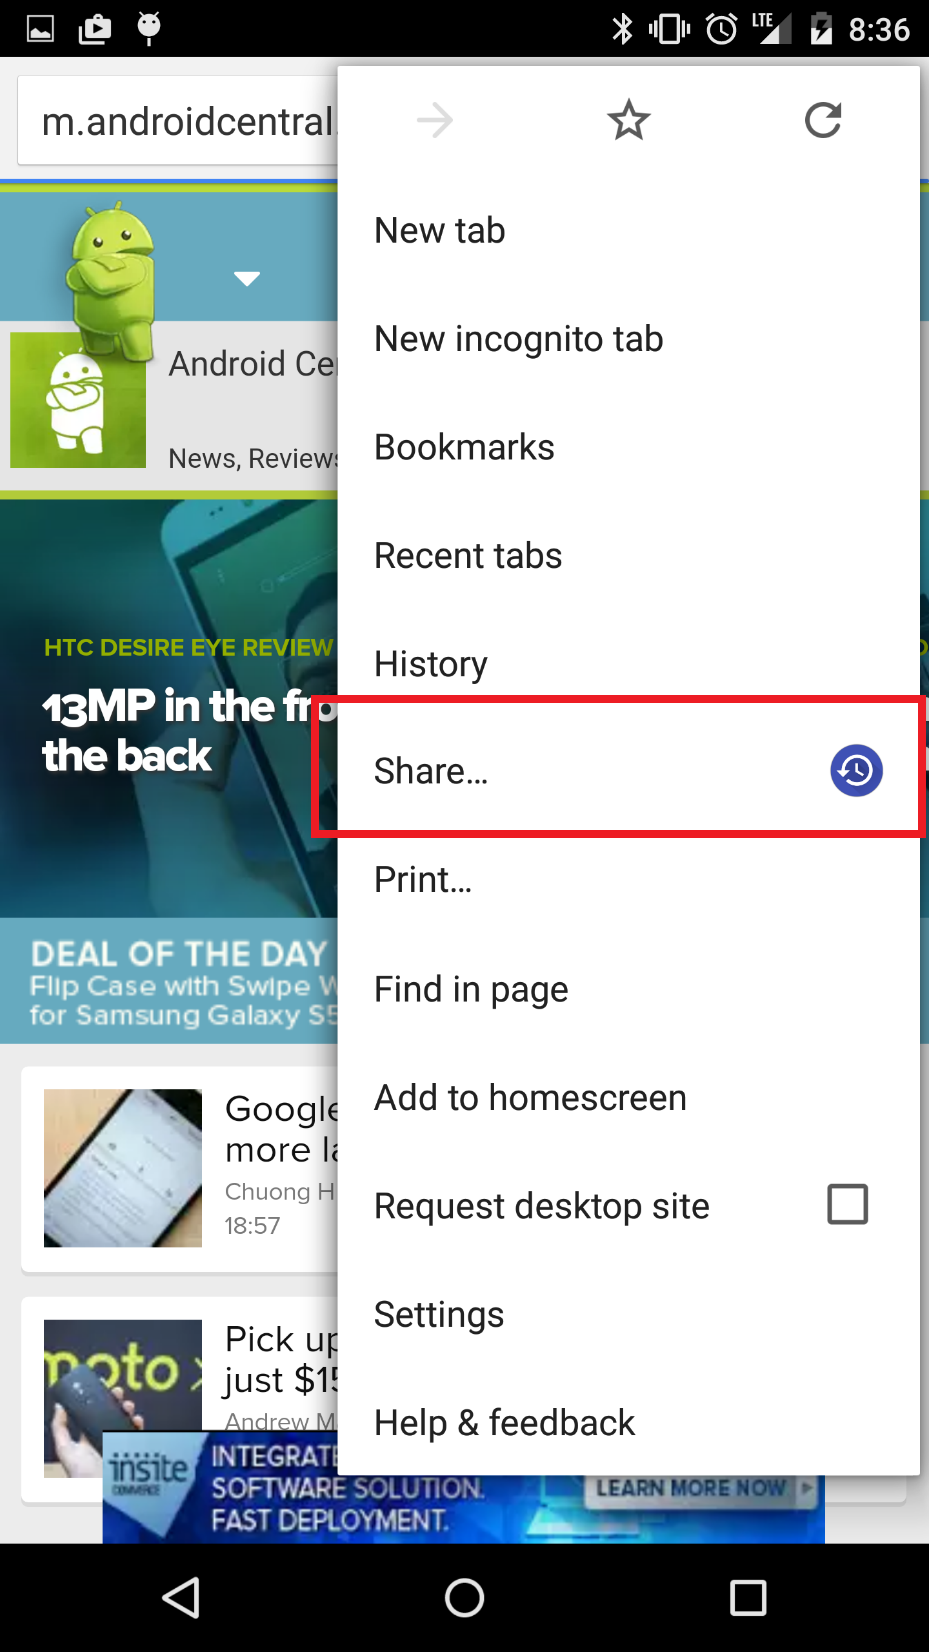
\includegraphics[width=0.21\textwidth]{./imgs/share.png}}\qquad
    \subfigure[Users may select the option of viewing the mementos of the currently viewed page.]{\label{mems}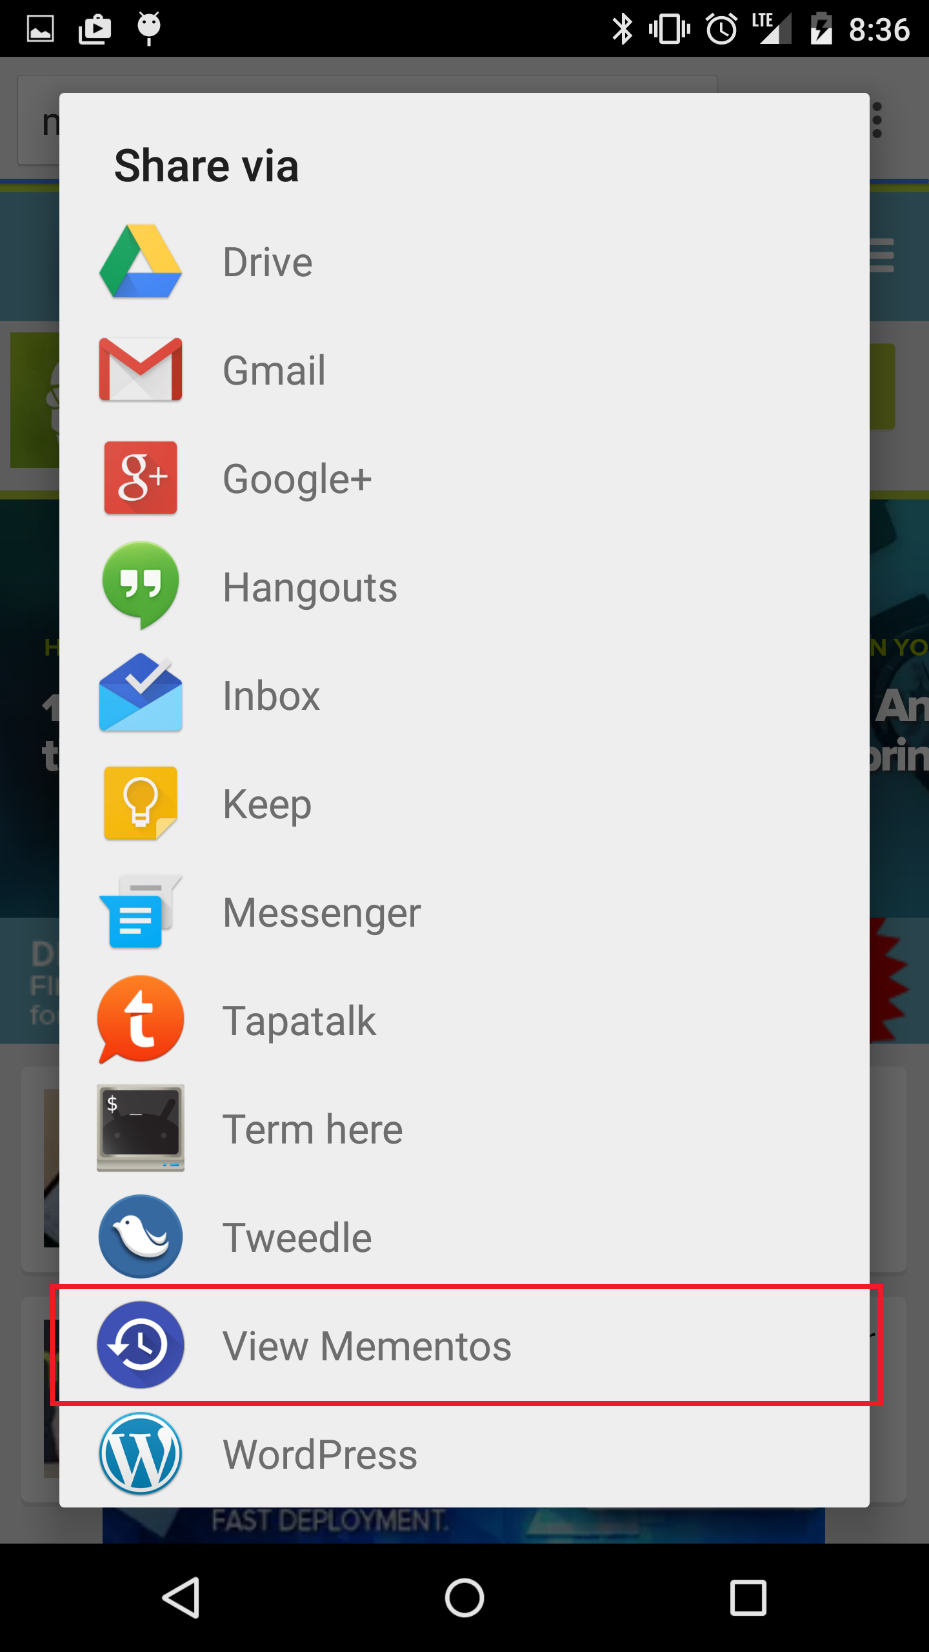
\includegraphics[width=0.21\textwidth]{./imgs/viewmems.png}}  \qquad
    \subfigure[The TimeMap consists of both mobile and desktop mementos.]{\label{tm}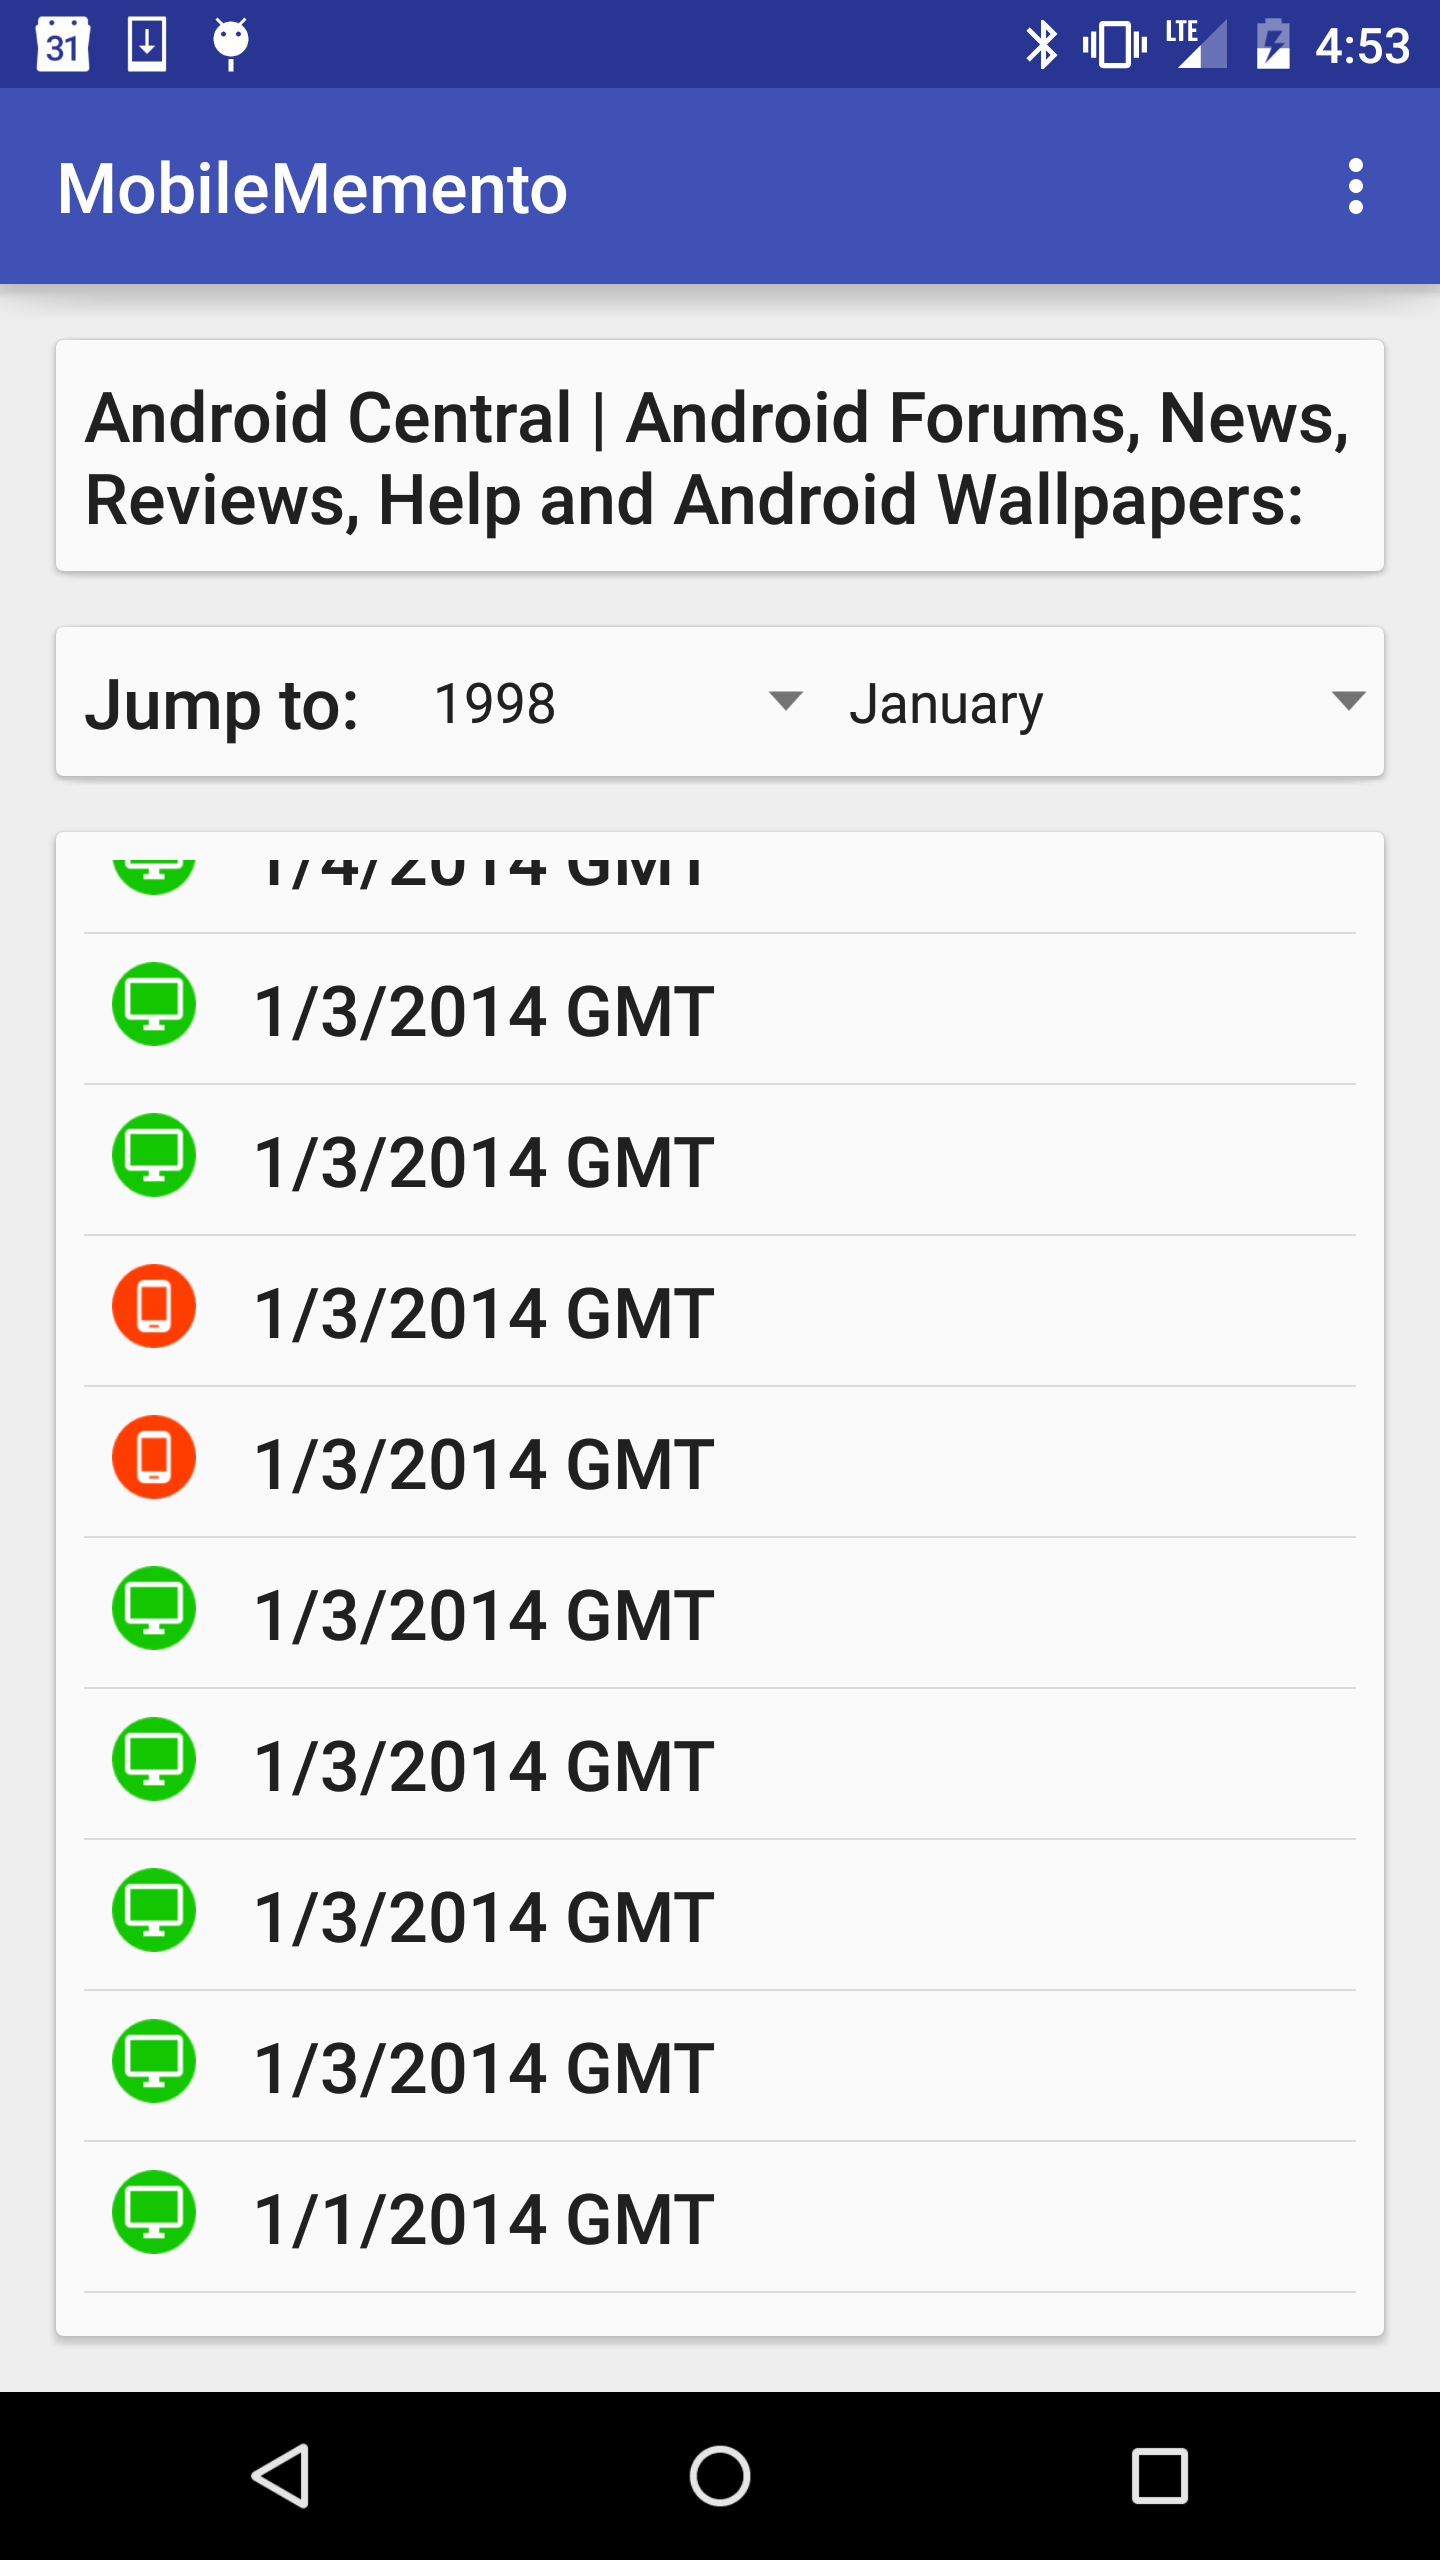
\includegraphics[width=0.21\textwidth]{./imgs/timemap.png}}  \qquad
    \subfigure[Users can submit the mobile and desktop URIs to archival services.]{\label{submit}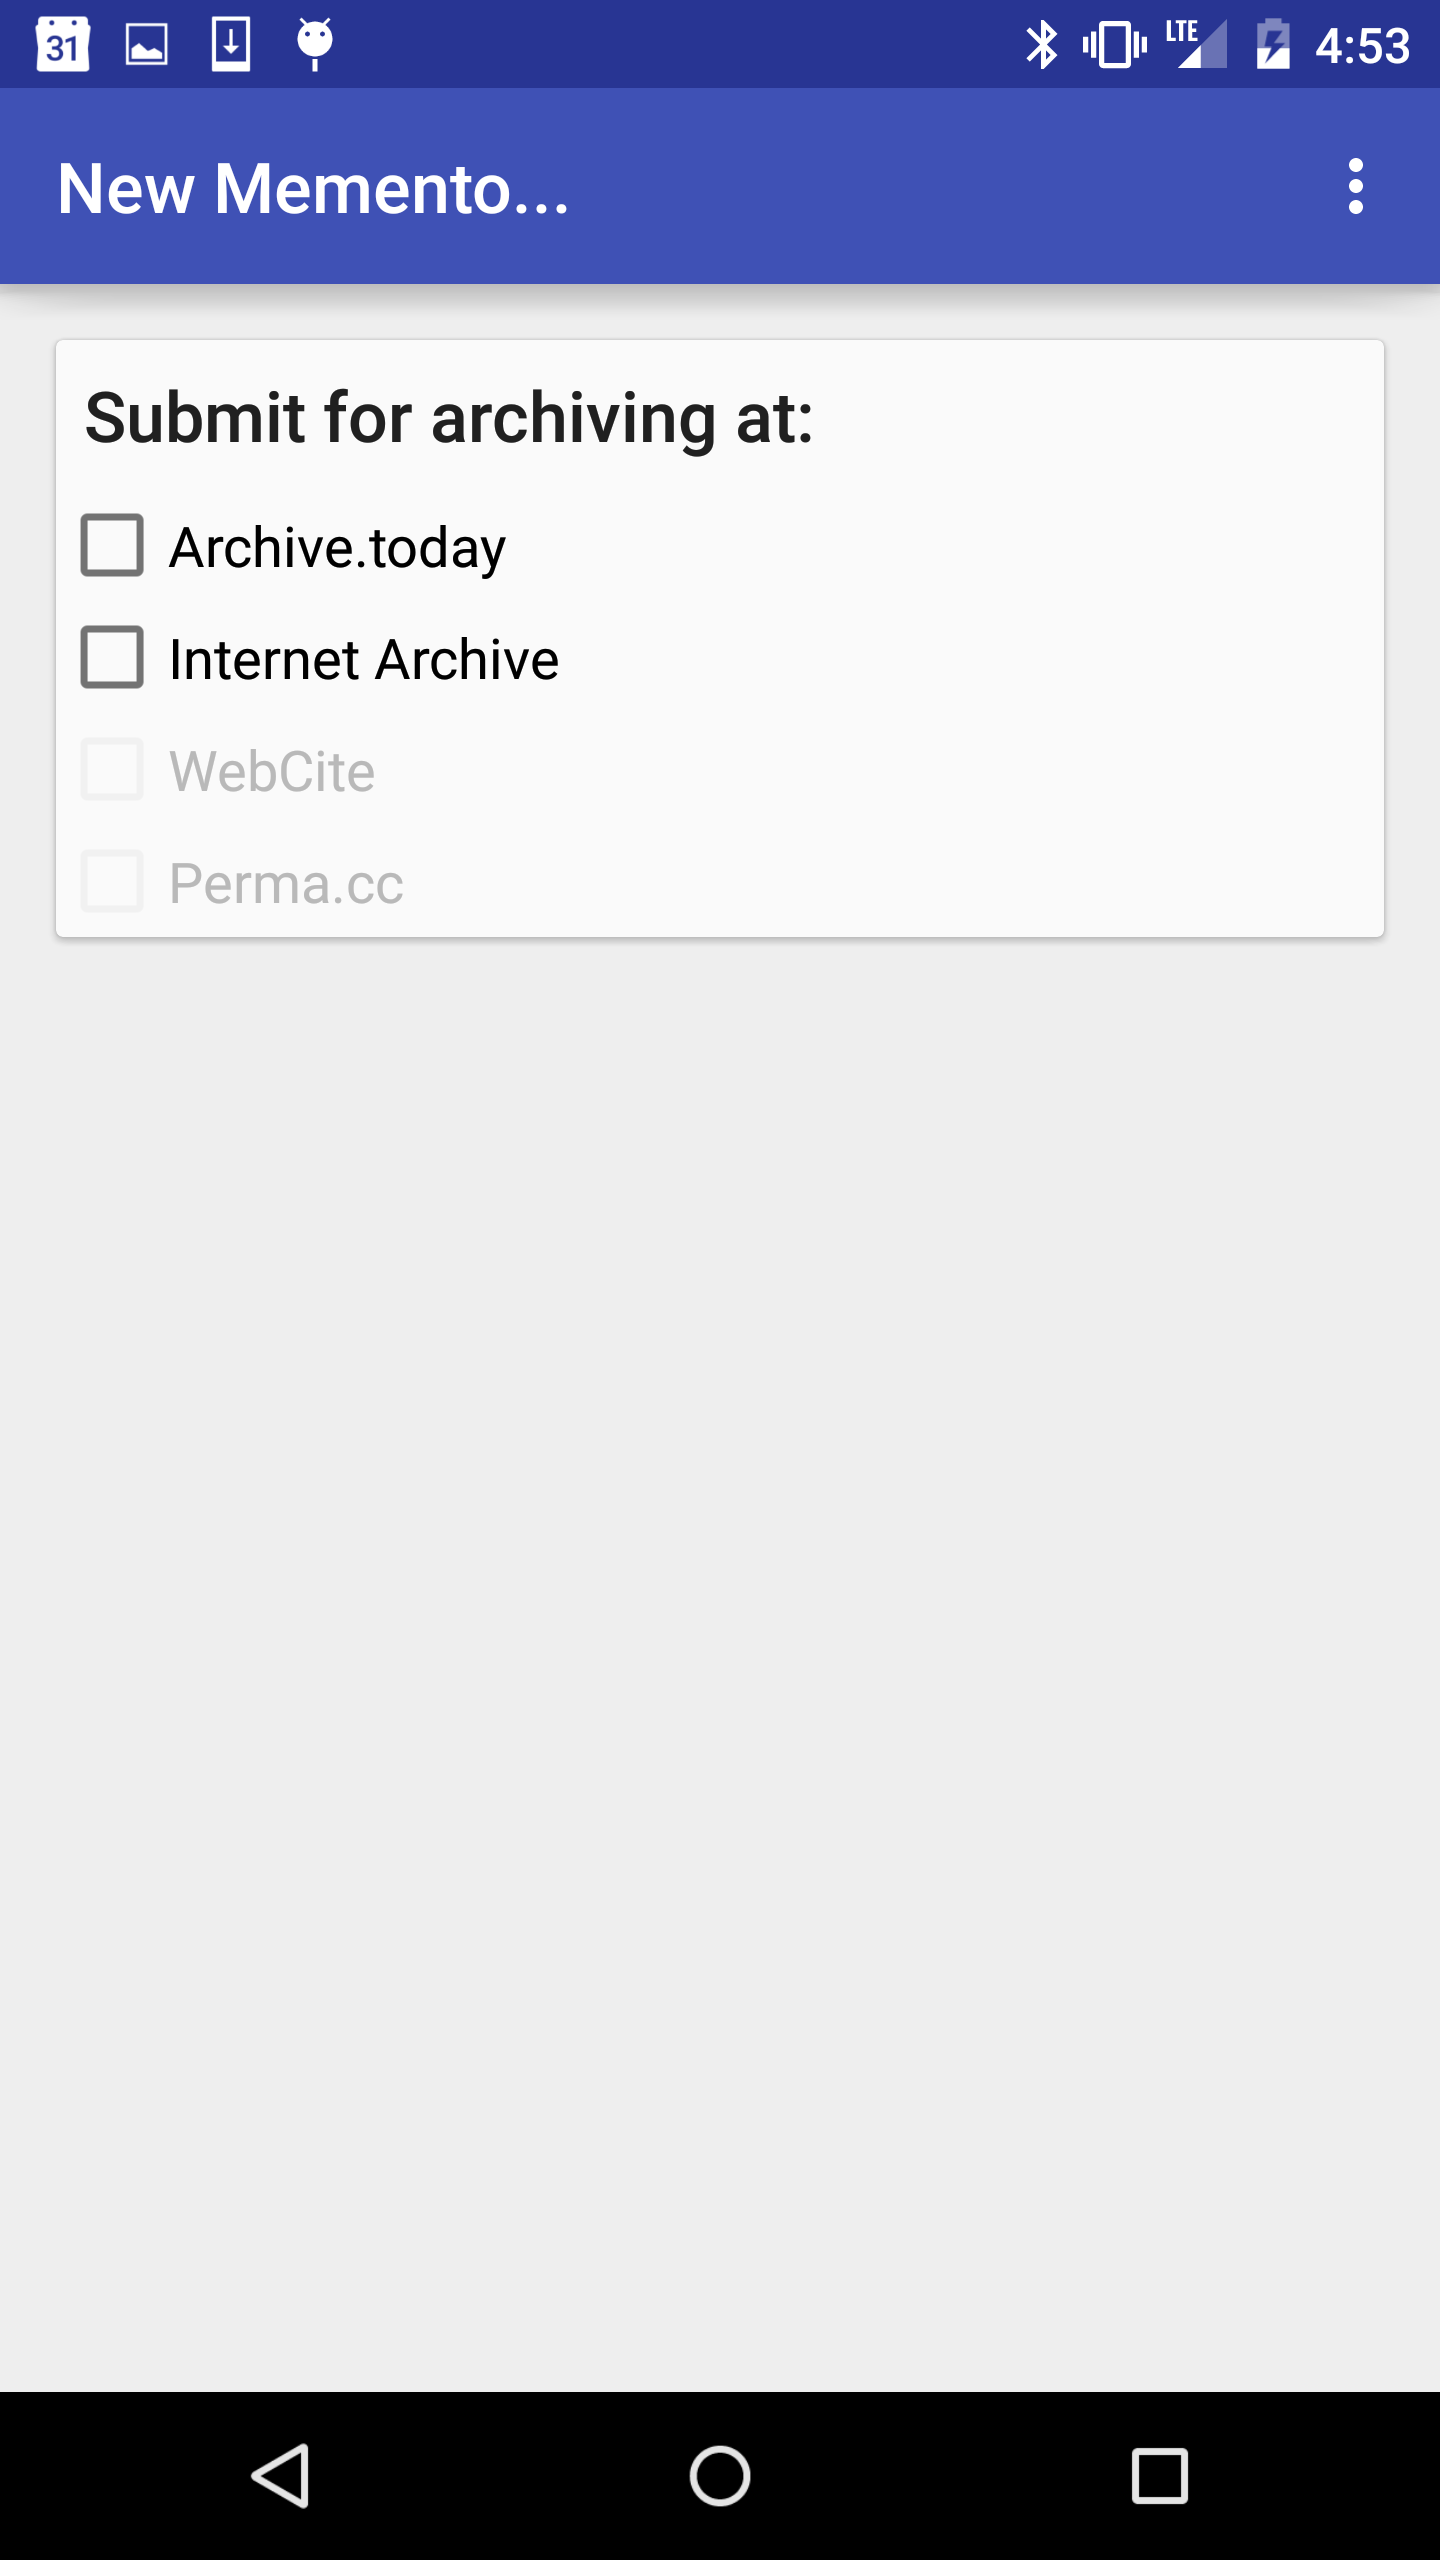
\includegraphics[width=0.21\textwidth]{./imgs/submit.png}}  
  \caption{Using existing Android browser features to view the TimeMap of the currently viewed page.}
  \label{clicks}
\end{figure*}

Mobile Mink is an Android application that is currently in development and will be released for download in the Google Play app store.
Much like its desktop browser parent, Mobile Mink offers a TimeMap of mementos that allows the user to navigate between the past and present webs. Mobile Mink also allows the user to submit mobile and desktop URI-Rs to be archived by archival services.

When using a web browser native to the Android operating system, the user is presented with an expandable menu in the top right of the browser window (called a ``view as list''). Selecting this sign opens a menu of options, one of which is the option to ``Share'' the page (Figure \ref{share}). Mobile Mink adds the option to ``View Mementos'' of the currently viewed page to the list of sharing options (Figure \ref{mems}).

Selecting the option of viewing mementos begins the process of discovering mobile and desktop URIs of the current URI-R. First, Mobile Mink identifies the URI-R of the currently viewed page. Mobile Mink identifies the URI-R as either a desktop URI or a mobile URI. Second, if the URI is a desktop URI, Mobile Mink translates the URI to a mobile URI; if the URI is a mobile URI, Mobile Mink translates the URI to a desktop URI. We use the same URI modifications as in Schneider and McCown's work \cite{frankMobile} and test for the mobile URI's existence on the live web (i.e., returns an HTTP 200 response) and in the archives (returns a TimeMap of cardinality $> 0$ from the Memento aggregator).

Note that our previous research demonstrated that differentiating between the mobile and desktop versions of a page can be difficult if the same URI is used to identify the mobile and desktop representations, and only content-negotiation based on the user-agent is used by the server to decide whether to return a mobile or desktop representation \cite{idReps}. Content-negotiation is out of the scope of this work, and we focus solely on differentiations by URI. Other methods of mobile representation discovery are available \cite{frankMobileDlib}.

With the URI-Rs of the mobile and desktop resources identified, we get the TimeMaps of both URI-Rs\\ (e.g., \url{m.androidcentral.com/} and \\\texttt{www.androidcentral.com/}). Mobile Mink compiles an aggregate TimeMap of both mobile and desktop mementos that is sorted by archival datetime and has icons indicating the mobile and desktop mementos by a mobile phone and PC icon, respectively (Figure \ref{tm}). We include mementos of all permutations of mobile and desktop URIs in the TimeMap because the mobile URIs may have changed over time (e.g., migrating from m.example.com to mobile.example.com). Selecting a memento from the list redirects the user's browser to the URI-M.


\section{Archiving Mobile URI-Rs}
\label{flow}
To ensure both the mobile and desktop representations exist in the archives, Mobile Mink allows the user to submit both URI-Rs to the Internet Archive's Save Page Now service and Archive.today (Figure \ref{submit}). Before the submission, Mobile Mink ensures that both URI-Rs return an HTTP 200 when dereferenced on the live web to prevent the attempted archiving of resources that do not exist. 

With this utility, Mobile Mink offers a way for users to actively curate mobile versions of pages they visit, even when crawlers and archival services cannot find them. With this feature, users can help archive the mobile web.

%ACKNOWLEDGMENTS are optional
\section{Acknowledgments}
This work supported in part by the NEH HK-50181. This work was performed as part of Wesley Jordan's mentorship at The MITRE Corporation. The author's affiliation with The MITRE Corporation is provided for identification purposes only, and is not intended to convey or imply MITRE's concurrence with, or support for, the positions, opinions or viewpoints expressed by the author. 


\bibliographystyle{abbrv}
\bibliography{_mybibtex}  



\end{document}

%%%%%%%%%%%%%%%%%%%%%%%%%%%%%%%%%%%%%%%%%%%%%
%%%LaTeX useful templates that i always need:
%%%%%%%%%%%%%%%%%%%%%%%%%%%%%%%%%%%%%%%%%%%%%


%\begin{figure*}
%  \begin{center}
%    \subfigure[]{\label{}\includegraphics[width=0.3\textwidth,height=3cm,keepaspectratio]{./imgs/}}
%    \subfigure[]{\label{}\includegraphics[width=0.3\textwidth]{./imgs/}}  
%  \end{center}
%  \caption{}
%  \label{}
%\end{figure*}

%\begin{table*}
%\centering
%\begin{tabular}{ p{2cm} |  c | c |}
%    \hline
%	X&Y&Z\\
%\end{tabular}
%  \caption{}
%  \label{}
%\end{table*}

%\begin{equation}
%\label{uricomp}
%\begin{split}
%F= &max(\lvert \text{client-side parameters} \rvert,\\
%&\lvert \text{server-side parameters} \rvert) 
%\end{split}
%\end{equation}


%\begin{equation}
%\label{uricomp2}
%UC = \frac{\lvert Depth \rvert + F}{2}
%\end{equation}